\section{Sort}

\subsection{Implementazione}
L'algoritmo scelto per l'ordinamento è il selection sort. L'algoritmo prevede di scambiare 
ogni elemento della lista con l'elemento più piccolo tra gli elementi successivi per ogni 
posizione della lista. È adatto all'uso nelle liste concatenate dato che non si effettua 
mai l'accesso diretto ad una certa posizione ma si scorre sempre gli elementi. 
Sono quindi definite le seguenti funzioni:

\begin{itemize}
    \item \textit{getMinAddress} che restituisce l'indirizzo del nodo più piccolo tra i nodi successivi
    al nodo specificato. 
    \item \textit{sort} che scambia un nodo con il risultato di \textit{getMinAddress}.
\end{itemize}
Entrambe le funzioni sono implementate ricorsivamente.
\subsection{Funzione getMinAddress}
La funzione getMinAddress ha due parametri, 
\textbf{a0} è l'indirizzo del nodo corrente, \textbf{a1} è l'indirizzo del nodo con il valore minimo.
La funzione confronta i valori dei due nodi, se il nodo corrente è minore del minimo allora il nodo minimo diventa il nodo corrente.
Dopo di che, controlla se il nodo corrente ha un nodo successivo, in caso non ci sia la funzione ritorna. Mentre se il nodo successivo è presente
la funzione si richiama sostituendo al nodo corrente il nodo successivo.
\\

\begin{lstlisting}[language=java,caption={Codice java algoritmo getMinAddress},captionpos=b] 
    private Node getMinAddress(Node current, Node min){
        if(current.getValue() < min.getValue()){
            min = current;
        }
        if(current.getNext() != null){
            min = getMinAddress(current.getNext(), min);
        }
    }
\end{lstlisting}

\subsection{Funzione sort}
La funzione sort ha un solo parametro, \textbf{a0} l'indirizzo nodo da sostituire con il minimo.
La funzione chiama \textit{getMinAddress} sul nodo corrente, e lo scambia con il risultato della funzione.
Dopo di che, controlla che ci sia il nodo successivo e in caso sia presente richiama la funzione \textit{sort} sul prossimo nodo.
\\
\begin{lstlisting}[language=java,caption={Codice java algoritmo sort}, captionpos=b]
    private void sort(Node current){
        Node min = getMinAddress(current, current);
        swap(current, min);
        if(current.getNext() != null){
            sort(current.getNext());
        }
    }
    
\end{lstlisting}

\subsection{Criteri di ordinamento}
\paragraph{Descrizione}
Il programma non ordina i nodi in base al valore ASCII, ma ha un ordinamento specifico:
\begin{itemize}
    \item Lettere Maiuscole ASCII(da 65 a 90 compresi)
    \item Lettere Minuscole ASCII(da 97 a 122 compresi)
    \item Numeri ASCII(da 48 a 57 compresi)
    \item Tutti gli altri simboli
\end{itemize}
All'interno dei gruppi gli elementi sono ordinati in base al loro valore ASCII.

\paragraph{Implementazione}
Per fare questo ordinamento associamo ad ogni valore ASCII un valore di ordinamento, 
di modo che gli elementi possano essere ordinati in base al loro valore di ordinamento.
Abbiamo perciò bisogno di una funzione che associa un numero ad ogni carattere di modo che:\\
Lettere Maiuscole $>$ Letter Minuscole $>$ Numeri $>$ Resto.
\\
Per fare questa funzione quello che facciamo è sommare un certo valore in base al gruppo di apparentenza di un carattere.

\begin{table}[H]
    \begin{center}
        \begin{tabular}{|c|c|c|c|}
            \hline
            Caratteri & Valore ASCII & Valore da sommare & Valore restituito \\
            \hline
            A-Z & 65-90 & 97 & 162-187 \\
            \hline
            a-z & 97-122 & 39 & 136-161 \\
            \hline
            1-9 & 48-57 & 78 & 126-135 \\
            \hline
            Resto & 32-125 & 0 & 32-125 \\
            \hline
        \end{tabular}
    \end{center}
    \caption{Tabella valore ordinamento}
    \label{tab:orderingValue}
\end{table}


Come possiamo vedere da Tabella \ref{tab:orderingValue} il valore restituito dopo la somma permette
di determinare facilmente l'ordine degli elementi.

Per semplicità di utilizzo la funzione \textit{getOrderValue} prende due elementi per volta (\textbf{a0},\textbf{a1}),
dato che ogni volta che la chiamiamo dobbiamo eseguire un confronto tra due elementi.
Essa ritorna il valore di ordinamento dei due elementi (\textbf{a0},\textbf{a1}). 

\subsection{Funzione swap}

\paragraph{Descrizione}
 La funzione \textit{swap} scambia di posizione due elementi della lista.
\paragraph{Implementazione} 
La funzione ha come parametri (\textbf{a0},\textbf{a1}) gli indirizzi dei due nodi.
Essa legge il dato di ogni nodo e scrive il valore del primo nel secondo e viceversa.
Scambiando il dato dei nodi dobbiamo effettuare 2 letture e 2 scritture, mentre se volessimo
scambiare i puntatori dovremmo effettuare ben 6 letture e 6 scritture, dato che dovremmo cambiare i due puntatori 
dei due nodi interessati e il puntatore al prossimo elemento dell'elemento precedente e il puntatore all'elemento precedente 
dell'elemento successivo. Come mostrato in Figura~\ref{fig:swap}. Pertanto dato che il dato è di un solo byte, mentre
i puntatori sono una word ciuascuno conviene scambiare i dati e lasciare i puntatori intatti.


\begin{figure}[h]
    \centering
    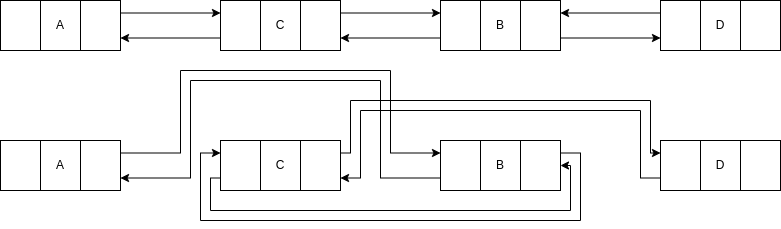
\includegraphics[scale=0.4]{diagrams/swap.png}
    \caption{Prima e dopo ordinamento con scambio di puntatori}
    \label{fig:swap}
\end{figure}

